\documentclass[bibliography=totoc]{scrartcl}
\usepackage[ngerman, english]{babel}
\usepackage{rwukoma}
\usepackage[pdfusetitle]{hyperref}
\usepackage{lipsum,caption}
\usepackage{acronym}
\usepackage{algorithm, algpseudocode}
\usepackage{graphicx}
\usepackage{subcaption}
\usepackage{listings}
\usepackage{float}
\usepackage{todonotes}
\usepackage{amsmath}
\usepackage{comment}

\setlength{\belowcaptionskip}{5pt}

\title{Comparison of different path planning algorithms}
\author{Manuel Gnannt - 34946, IN \\ Florian Betz - 35653, IN}
\date{13.03.2023}%\today}
\begin{document}
\maketitle
\tableofcontents

\clearpage
\section{Abstract}
In path planning, discovering good trajectories often requires a high-dimensional model and the evaluation of many samples. Recently, Wang et al. proposed an algorithm called \textbf{La}tent Space \ac{LaP3} claiming it outperforms existing path planning methods in 2D navigation tasks with respect to sample efficiency. In this paper, we compare the newly published \ac{LaP3} to other path-planning algorithms in several 2D environments.
\todo[inline]{extend descriptions with all information, Florian}
%\todo[inline]{problems, why, solutions, results}

\section{Introduction}
In path planning, the goal is to find the most rewarding trajectory in a given search space. 

A common problem faced by approaches like CMA-ES \cite{CMA-ES} is being trapped at local optima. 
Another is the exploration-exploitation tradeoff. 
Approaches like VOOT \cite{VOOT} try to tackle both the local optimum problem and the exploration-exploitation tradeoff by partitioning the search space.
This partitioning however is done independently from the reward function, making it less efficient.

For a more efficient search space partitioning, Wang et al. proposed \ac{LaP3} an extension of \ac{La-MCTS} \cite{La-MCTS} where the search space is  partitioned into high- and low-reward regions thus splitting is done based on the reward function.
%The main difference between \ac{LaP3} and \ac{La-MCTS} is a different calculation of the node values and additional sampling via CMA-ES instead of Bayesian Optimization.

This paper explores the topic of path planning, with a focus on three specific algorithms A*, \ac{La-MCTS}, and \ac{LaP3}. 
\begin{comment}

\ac{LaMCTS} and \ac{LaP3}, on the other hand, are more recent algorithms that have been developed to address specific challenges in path planning, such as handling large or complex environments.
\end{comment}

\newpage
\section{Path Planning Algorithms}
\label{path_planning_algorithm}
In this paper, we decided to use three different search algorithm A*, \ac{La-MCTS} and \ac{LaP3}.

\subsection{A*}
%\todo[inline]{image? Zitat, Florian}
%\todo[inline]{Seite + Zeilen zu jedem Zitat (Text und image), Florian}

The A* algorithm, first introduced by Peter Hart and other researchers at the Stanford Research Institute in 1968, is a widely used method for pathfinding and graph traversal. \cite{4082128} It builds on Dijkstra's algorithm by incorporating heuristic functions and predicted costs, making it the most efficient direct search method for finding the shortest paths in a static road network and a popular heuristic for various other problems.\cite{ProbabilisticApproachCollaborativeMultiRobotLocalization}

The key component of the algorithm is the design of the valuation function, $f(n) = g(n) + h(n)$, where $g(n)$ is the actual cost from the initial node to node n, $h(n)$ is the estimated cost from node n to the target node, and $f(n)$ is the estimated cost from the initial node via node n to the target node. The A* algorithm can reach a time complexity of $O(n)$.

\textbf{Step 1:} Add the starting node to the priority queue.
\newline
\textbf{Step 2:} Select the node with the smallest F-value from the current priority queue and make it the current node.
\newline
\textbf{Step 3:} Mark it as visited and process its adjacent nodes.
\newline
\textbf{Step 4:} If the neighboring node has not been visited, add it to the queue, set the current node as its parent, and record its F, H, and G values. If the neighboring node has already been visited, check if the current node has a shorter path by comparing G values. If the current node has a smaller G value, update the parent node and G, H values of that node.
\newline
\textbf{Step 5:} Repeat steps 2 to 4 until the target node is marked or the priority queue is empty.
\newline
\textbf{Step 6:} When the path is found, trace back from the endpoint to the start node using the parent node.



\begin{figure}[H]
	\centering
	\begin{subfigure}[b]{0.3\linewidth}
		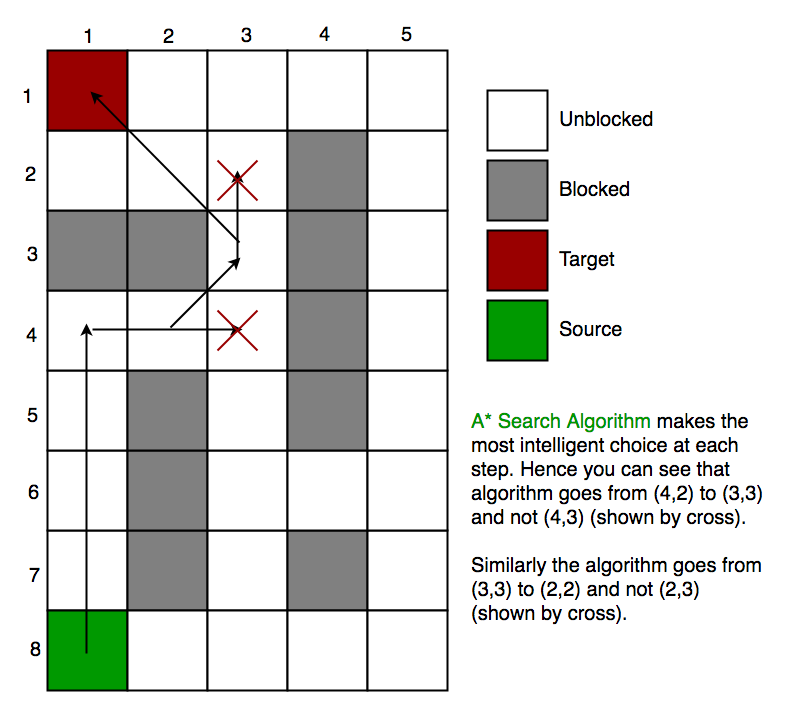
\includegraphics[width=\linewidth]{img/a_-search-algorithm.png}
        \caption{Astar path}	
    \end{subfigure}
	\hspace{0.02\textwidth}
	\begin{subfigure}[b]{0.3\linewidth}
		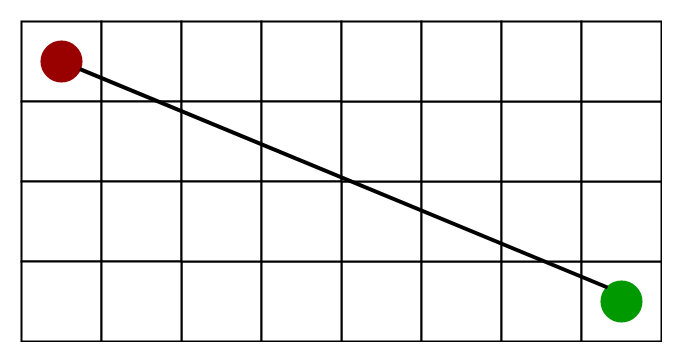
\includegraphics[width=\linewidth]{img/a_-search-algorithm-euclidian_distance.png}
		\caption{Euclidean Distance Heuristics}
	\end{subfigure}
 	\caption{Astar \cite{Pic:astar}}
	\label{fig:differentenvironments}
\end{figure}

\begin{comment}
    

\subsection{Monte-Carlo Tree-Search}
\todo[inline]{unbedingt notwendig?}
The leaves in the monte-carlo tree represent different states in a search space. The links to different children of a leaf represent different actions to get to a different state.

\begin{figure}[H]
	\centering
	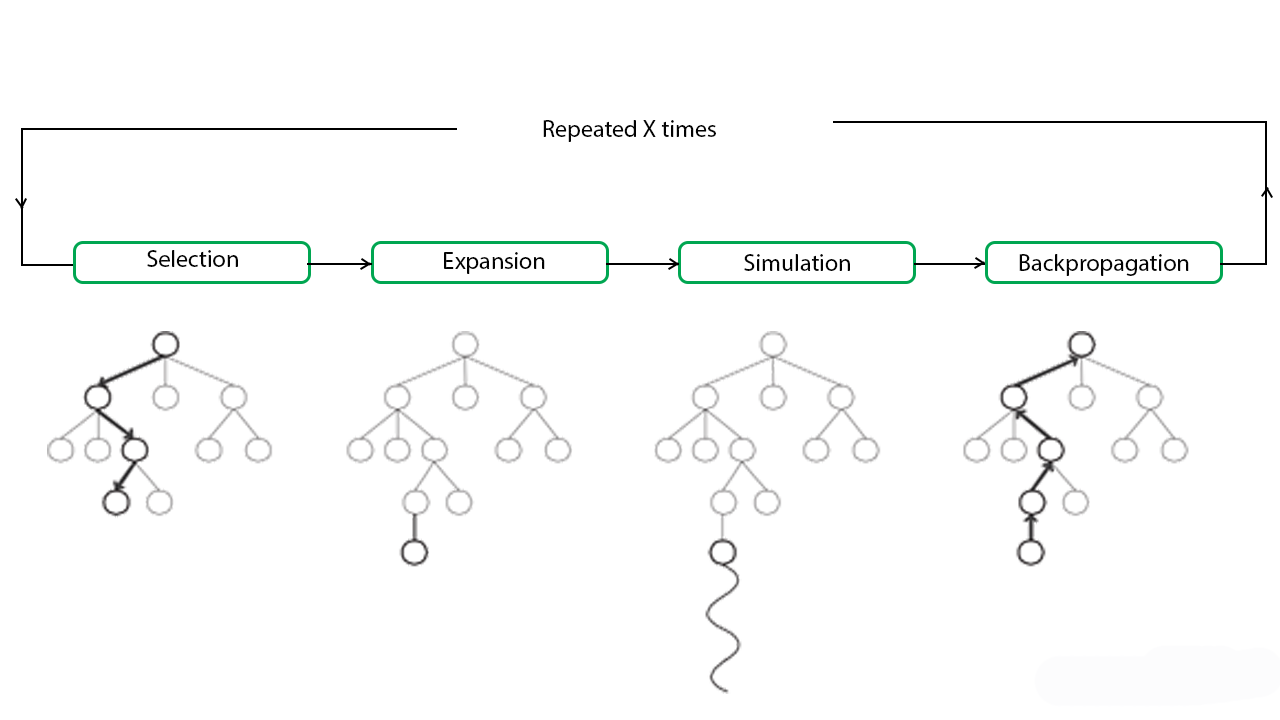
\includegraphics[width = {\textwidth}]{img/mcts_steps.png}
	\caption{Steps of \ac{MCTS}}
	\label{fig:MCTS}
\end{figure}

The tree now learns by performing the following steps:

\textbf{Step1: Selection} When in a given state, an appropriate action is selected based on a policy.

\textbf{Step 2: Expansion} When the selected leaf does not have any children, different actions are performed which lead to additional nodes.

\textbf{Step 3: Simulation} The reward of the newly created leaves is calculated and the best nodes are added to the tree.

\textbf{Step 4: Backpropagation} All nodes above the selected one are updated based on the reward they lead to.
\end{comment}
\newpage
\subsection{La-MCTS}
The basic idea of a Latent Action Monte-Carlo Tree-search (La-MCTS) is to recursively split the search space with every region representing a node in a Monte-carlo tree.\cite{La-MCTS}
As shown in figure \ref{fig:laMCTS_sampling_plitting}, this is done by taking some samples from the search space and splitting it into a high- and a low-reward section using K-means(k=2). 
An SVM then learns this boundary and the two sections can be represented as nodes in a monte carlo tree.
In our example, the high-reward section is represented by the left node and the low-reward section by the right node.


\begin{figure}[H]
	\centering
	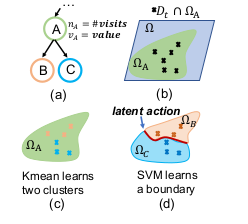
\includegraphics[width = {0.35\textwidth}]{img/lamcts_1.png}
	\caption{\ac{La-MCTS} sampling and splitting \cite{La-MCTS}[p.3]}
	\label{fig:laMCTS_sampling_plitting}
\end{figure}
As shown in in figure \ref{fig:laMCTS_workflow}, this process is now repeated by selecting a node until a leaf node is reached, taking samples along the corresponding section and splitting it again. 
This results in a tree structure with the leftmost node representing the section with the highest reward. 

\begin{figure}[H]
	\centering
	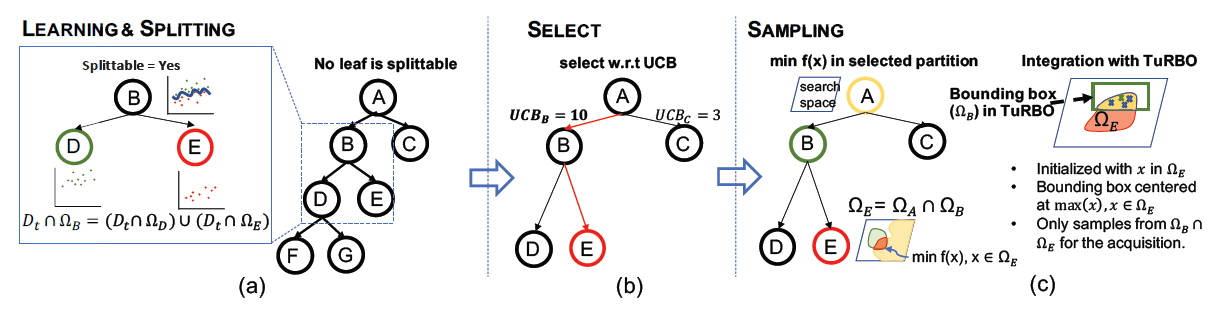
\includegraphics[width = {\textwidth}]{img/lamcts_workflow.png}
	\caption{Steps of \ac{MCTS} \cite{La-MCTS}[p.4]}
	\label{fig:laMCTS_workflow}
\end{figure}

\begin{comment}
    

In a Latent space Monte-Carlo Tree-search, the search space is partitioned into a high- and low-reward section using K-means (k=2) and an SVM learning the boundary. These sections are represented as nodes in a monte-carlo tree. The value of each node

This is done by creating a dataset consisting of (x, f few samples and splitting the search space in a high-reward partition and a low-reward partition using K-means(k=2) and an SVM learning the boundary. These partitions are represented by two child nodes in the monte-carlo tree. In a next step, samples are taken from around each cluster center and based on these samples, the now child-node is partitioned again in a high- and low-reward region. This results in a monte carlo tree with the left-most leaf being the highest-reward region, the leaf left to the highest one being the second-highest and so on.

\end{comment}


\subsection{LaP3}
%https://www.youtube.com/watch?v=-4Lzk_s_Dzw
\ac{LaP3} The search space is partitioned into regions by drawing samples and recursively splitting by reward. The value/UCB of a node is calculated using the maximum value instead of the mean.(formula) Afterwards a path to the child nodes is planned using CMA-ES\cite{CMA-ES}.
\cite{NEURIPS2021_03a3655f}
It is a new path planning method which improves the function value estimation within each sub-region.
This algorithm use a latent representation of the search space.
\ac{LaP3} and \ac{La-MCTS} use the maximum, instead of the mean, as the node score to improve sample efficiency.

\todo[inline]{Text und Bilder + Formeln aus dem Paper, Manuel}

\newpage
\section{Methodology}
We ran \ac{LaP3}, \ac{La-MCTS} and an A* on two different environments with both environments containing local optima. For each environment, the experiment was run on a 12x12, a 24x24 and a 36x36 grid. As the goal is finding a sample efficient trajectory the number of samples was used as a metric in relation to the reward. The reward was calculated by the inverse of the euclidian distance to the target. It can be described by following formula. 

\begin{equation}
\left\{
\begin{array}{lll}
 r(\vec{x})=\frac{10}{\sqrt{\Delta x_1 ^2+\Delta x_2 ^2}}\quad \Delta x_1 + \Delta x_2 \neq 0\\
r(\vec{x})=15\quad \Delta x_1 + \Delta x_2 =0\\
\end{array}
\right.
\end{equation}

\begin{figure}[H]
	\centering
	\begin{subfigure}[b]{0.3\linewidth}
		\includegraphics[width=\linewidth]{img/Maze_s3.png}
        \caption{Maze S3 environemt}	
    \end{subfigure}
	\hspace{0.02\textwidth}
	\begin{subfigure}[b]{0.3\linewidth}
		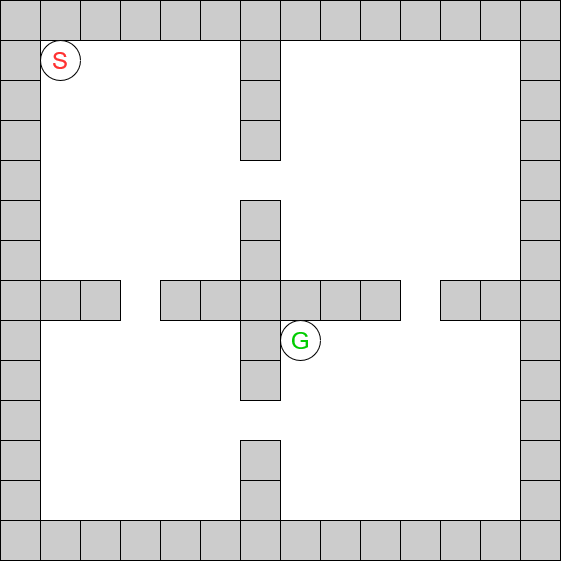
\includegraphics[width=\linewidth]{img/Four_Rooms.png}
		\caption{Four Rooms}
	\end{subfigure}
 	\caption{different environments}
	\label{fig:differentenvironments}
\end{figure}

\todo[inline]{four rooms change target position, replace right image, Florian}

\subsection{Search Efficiency}
The goal in path planning is to find the most rewarding trajectory in the search space.
As the optimum can eventually be found by random sampling if the number of samples is high enough, an efficient algorithm is preferred.
The search efficiency of an algorithm can therefore be described by the number of samples and the achieved reward.
As this metric is used widely when comparing different search algorithms, \cite{La-MCTS}, \cite{LaNAS}, \cite{VOOT}, we also used it for comparison.

\todo[inline]{LaNas wird als Acronym nicht verwendet}



\newpage
\section{Evaluation}

%1. LaP3 Algorithmus wurde entwickelt, der die Pfade schneller berechnet
%2. LAP3 performt besser als der MCTS und A*
%3. Anhand gleicher Anzahl an samples ist der reward beim LAP3 immer besser
%4. verschiedene Metriken wurden verwenden space complexity, world environment
%5. Was sind unsere Ergebnisse, Performt LAP3 tatsächlich immer besser?
%6. Was kann in Zukunft noch nageschaut werden?

With the evaulation criteria and the different environment, the search algorithms are examined to see if the \ac{LaP3} performs better from several points of view.
Figure \ref{fig:SampleRewardMazeDifferentSpaceComplexity} shows the number of samples drawn and the associated reward in different environments with different complexities.
The environment is the maze s3 with complexity size 12x12, 24x24 and 36x36
The A* always delivers the same results, but \ac{La-MCTS} and \ac{LaP3} deliver different results on hundred runs and 
That is why the mean value and the lower and upper bound of the 95\% confidence interval are displayed in the graphs.
It can be seen that the \ac{LaP3} gets a larger reward than the \ac{La-MCTS} and A* with the same number of samples.
Although the \ac{LaP3} has a high variance, the reward increases consistently with increasing samples.
However, the \ac{LaP3} algorithm has a very large scattering of the delivered results.
For the \ac{La-MCTS}, an increase in variance does not occur until a sample size of 42 in a 12x12 environment and a sample size of 55 in a 24x24 and 36x36 environment.
The reward from the A* fluctuates continuously, but the reward does not increase as the number of samples increases.

\begin{figure}[H]
	\centering
	\begin{subfigure}[b]{0.3\linewidth}
		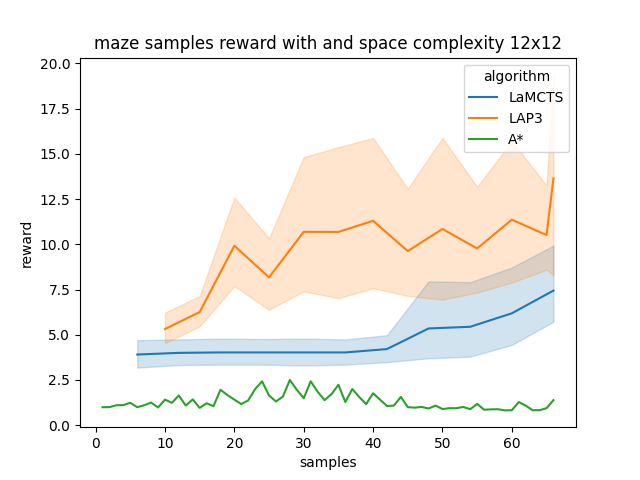
\includegraphics[width=\linewidth]{img/maze_samples__reward_b_8_LAP3_MCTS_AStar_interrupted_12.png}
        \caption{space complexity 12x12}	
    \end{subfigure}
	%\hspace{0.02\textwidth}
	\begin{subfigure}[b]{0.3\linewidth}
		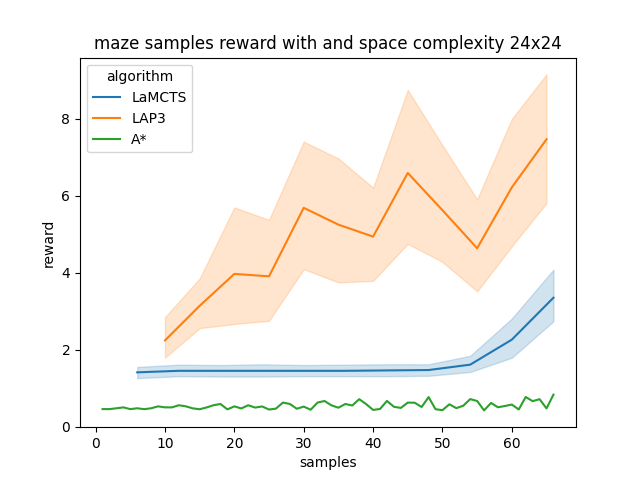
\includegraphics[width=\linewidth]{img/maze_samples__reward_b_8_LAP3_MCTS_AStar_interrupted_24.png}
		\caption{space complexity 24x24}
	\end{subfigure}
	%\hspace{0.02\textwidth}
	\begin{subfigure}[b]{0.3\linewidth}
		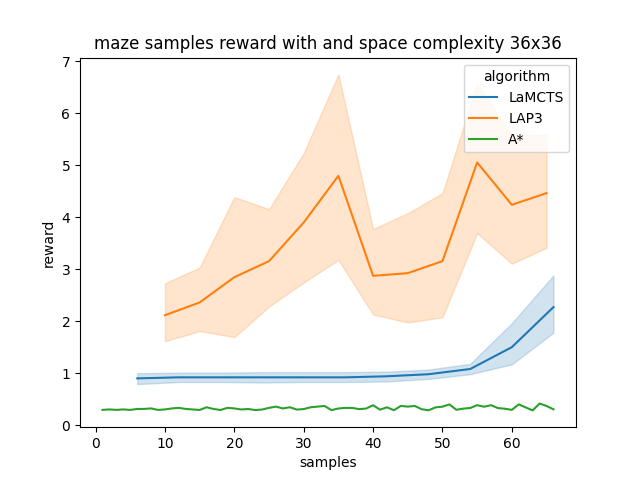
\includegraphics[width=\linewidth]{img/maze_samples__reward_b_8_LAP3_MCTS_AStar_interrupted_36.png}
        \caption{space complexity 36x36}
	\end{subfigure}
	\caption{ratio of samples and reward in Maze s3 environment with different space complexity}
	\label{fig:SampleRewardMazeDifferentSpaceComplexity}
\end{figure}

Figure \ref{fig:SampleRewardFourRoomsDifferentSpaceComplexity} shows the ratio of samples drawn and the associated reward in the four rooms environment with complexity size 12x12, 24x24 and 36x36.
As in the maze s3 environment, the A* generates a low reward with a low number of samples. 
Only in the 12x12 environent with a sample number of 40 does the reward increase and achieve a similar reward to the \ac{La-MCTS}.
With greater space complexity, the reward remains constantly low.
The \ac{La-MCTS} corresponds to a growing exponential function with constant mean.
The \ac{LaP3} on the other hand has a strong growth of the rewards at the beginning. With increasing sample number, however, the growth is reduced. However, the reward of \ac{LaP3} is larger than that of \ac{La-MCTS} and A* at each sample number.

\begin{figure}[H]
	\centering
	\begin{subfigure}[b]{0.3\linewidth}
		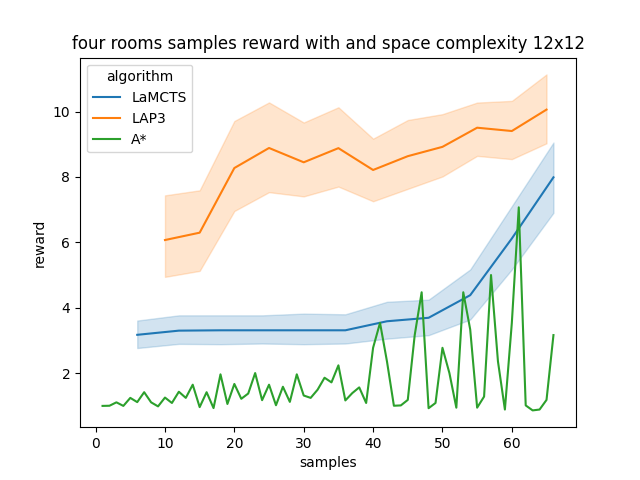
\includegraphics[width=\linewidth]{img/four_rooms_samples__reward_b_8_LAP3_MCTS_AStar_interrupted_12.png}
        \caption{space complexity 12x12}	
    \end{subfigure}
	\hspace{0.02\textwidth}
	\begin{subfigure}[b]{0.3\linewidth}
		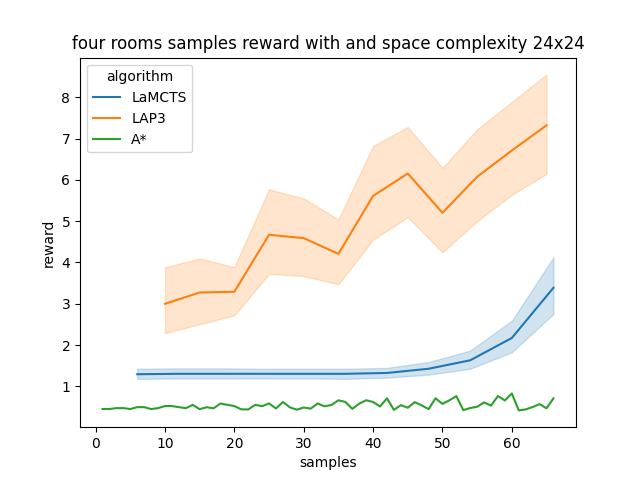
\includegraphics[width=\linewidth]{img/four_rooms_samples__reward_b_8_LAP3_MCTS_AStar_interrupted_24.png}
		\caption{space complexity 24x24}
	\end{subfigure}
	\hspace{0.02\textwidth}
	\begin{subfigure}[b]{0.3\linewidth}
		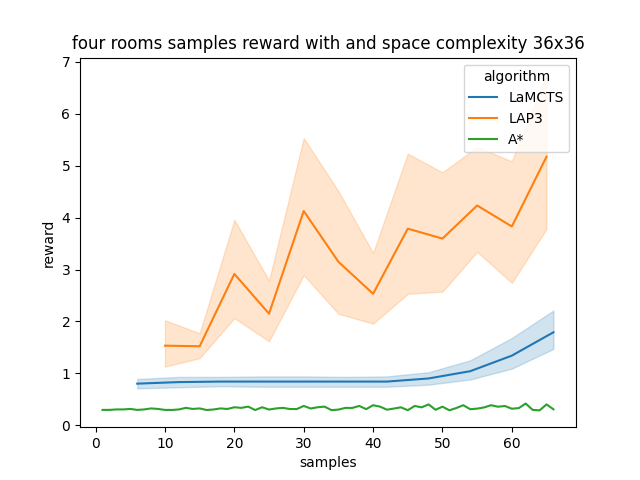
\includegraphics[width=\linewidth]{img/four_rooms_samples__reward_b_8_LAP3_MCTS_AStar_interrupted_36.png}
        \caption{space complexity 36x36}
	\end{subfigure}
	\caption{ratio of samples and reward in four rooms environment with different space complexity}
	\label{fig:SampleRewardFourRoomsDifferentSpaceComplexity}
\end{figure}

What is striking in both environments is that the \ac{LaMCTS} has a constant reward function. In the beginning, the reward is constant and increases exponentially after 40 samples.
The \ac{LaP3}

\begin{table}[H]
\centering
\begin{tabular}{|c|c|c|c|c|}
\hline
& {12x12} & {24x24} & {36x36} \\ \hline
Samples & $\overline{x}$ & $\overline{x}$ &  $\overline{x}$ \\ \hline
20 & 9.9208     & 3.9697  & 2.8462 \\ \hline
25 & 8.1711     & 3.9062  & 3.1538 \\ \hline
30 & 7.4318     & 2.4773  & 1.7554 \\ \hline
35 & 10.6842    & 5.25    & 4.7949 \\ \hline
40 & 11.3       & 4.9394  & 2.8718 \\ \hline
45 & 9.625      & 6.5938  & 2.9231 \\ \hline
50 & 10.8485    & 5.625   & 3.1538 \\ \hline
55 & 9.7692     & 4.6364  & 5.0513 \\ \hline
60 & 8.5443     & 3.2197  & 2.2536 \\ \hline
\end{tabular}
\caption{mean and 95\% confidence interval of \ac{LaP3} with different numbers of samples drawn in maze s3 environment}
\label{tab:mean_std_diff_sizes}
\end{table}



\begin{comment}
    
To improve the data dispersion in the \ac{LaP3} algorithm, the number of samples per region can be increased. In Figure \ref{fig:SampleRewardMazeDifferentSpaceComplexity}, 5 samples per region were drawn.

5 samples per region:
$\overline{x}$=8.4629
$\sigma$=4.2731 \newline
10 samples per region:
$\overline{x}$=7.9001
$\sigma$=4.2480 \newline
15 samples per region:
$\overline{x}$=9.0118
$\sigma$=4.7755

Changing the number of samples per region does not reduce the reward dispersion in the \ac{LaP3} algorithm.
\end{comment}
\todo[inline]{Aussage beantwortet, \ac{LaP3} performt immer besser}
%\todo[inline]{if lenyvec good größer 5 wie viele samples pro region immer beide ändern}


\section{Conclusions and Further Discussion}
Different sampling methods

\todo[inline]{What could be explorer in the future}

\todo[inline]{functions evals?, Manuel}
\todo[inline]{sample drawing in sequential action space (horiyon tto draw samples from, not whole search space), Manuel}

\clearpage


\section*{Acronyms} 
\addcontentsline{toc}{section}{Acronyms}

\begin{acronym}[....]
    \acro{LaP3}{Latent Space Partitions for Path Planning}
    \acro{MCTS}{Monte Carlo Tree Search}
    \acro{La-MCTS}{Latent Action Monte Carlo Tree Search}
    \acro{LaNas}{Latent Space Neural Architecture Search}
\end{acronym}

\bibliographystyle{alpha}
\bibliography{literature}
\end{document}
